%!TEX root = ../main.tex
\chapter{LITERATURE SURVEY}
\label{chap:intro}
In this section, I have categorized my literature survey into three parts namely link prediction, collective classification and network embedding with deep learning techniques. I started my survey by reading papers on different link prediction methods and implemented a paper which is explained in Section III. Then I read papers on collective classification and papers based on network embedding.

\section{\textbf{Non Destructive Evaluation (NDE)}}

Link prediction attempts to estimate the likelihood of the existence of a link between two nodes based on observed links and attributes of nodes. Given a graph,
\begin{align*}
G = (V , E)
\end{align*}
where $V$ is set of vertices and $E$ is set of edges between $V$, $U$ denotes set of all possible edges, $N = U - E$ denotes set of non-existent edges and $M \subset U$ represents missing or future edges, one has to find the missing or the future edges $M$. General problem in link prediction is the class imbalance between missing links with that of possible links. To solve using machine learning algorithms, one has to perform either sampling, active learning or cost-sensitive learning. Link prediction has many applications such as in biological networks where it is expensive to experimentally establish each link, spurious link detection where we need to remove those links from the network, link discovery problems like recommendation of products or friends to users, etc.

\begin{flushleft}
\textbf{The Link Prediction Problem for Social Networks \cite{linkpred} :}
\end{flushleft}

\indent This is the basic paper to address the link prediction problems and its solutions are categorized into proximity based link predictions, random walk based link predictions and matrix factorization based link predictions.

Proximity based Link Predictions : Proximity measure can be divided into local neighborhood and global path based approach. Local neighborhood approach is based on the neighborhood information available in the network. They capture similarities between nodes and they predict links such that more similar nodes typically form a link. Global path based approach calculates promixity of two nodes by capturing the paths between them in various ways in the network. Global path based approach is computationally expensive when compared to local neighborhood based approach as they may need to scan across the network if the two nodes are apart from each other.

Random Walk based Link Predictions : Performing random walk from a vertex captures the neighborhood information of that vertex. Two nodes can be similar if they are present in the random walk generated by those vertices. Random walks generated by the two vertices may not be same. 

Matrix Factorization based Link Predictions : The adjacency matrix can be factorized based on low rank approximation to represent the latent feature vectors in low dimensional space where the factorized matrix captures the information of users.

\begin{table}[ht!]
\begin{center}
\scalebox{1.5}{
\begin{tabular}{ |c|c| } 
 \hline
 Method & Formula  \\ 
 \hline 
 \hline
 Common Neighbors & $ |\Gamma(x) \cap \Gamma(y)|  $\\ 
 \hline
 Adamic/Adar & $ \sum_{z \in \Gamma(x) \cap \Gamma(y)}\frac{1}{log|\Gamma(z)|}  $\\ 
 \hline
 Resource Allocation & $ \sum_{z \in \Gamma(x) \cap \Gamma(y)}\frac{1}{|\Gamma(z)|}  $\\ 
 \hline
 Jaccard's Coefficient & $ \frac{|\Gamma(x) \cap \Gamma(y)|}{|\Gamma(x) \cup \Gamma(y)|}  $\\ 
 \hline
  Preferential Attachment & $ |\Gamma(x)| \cdot |\Gamma(y)|  $\\ 
  \hline
  Salton Index & $ \frac{|\Gamma(x) \cap \Gamma(y)|}{\sqrt{|\Gamma(x)| \cdot |\Gamma(y)|}} $\\
  \hline
  Sorenson Index & $ \frac{2|\Gamma(x) \cap \Gamma(y)|}{|\Gamma(x)| + |\Gamma(y)|} $\\
  \hline
  Hub Promoted Index & $ \frac{|\Gamma(x) \cap \Gamma(y)|}{min(|\Gamma(x) , \Gamma(y)|)}  $\\
  \hline
  Hub Depressed Index & $ \frac{|\Gamma(x) \cap \Gamma(y)|}{max(|\Gamma(x) , \Gamma(y)|)} $\\
  \hline
  Shortest Path & $ min{|p_{u->v}|}$ \\
  \hline
  Katz & $ \sum_{l=1}^{\infty}\beta_{l}|p_{u->v}^l|$\\
  \hline
\end{tabular}
}
\end{center}
\caption{Proximity based Link Prediction methods}
\label{table:3}
\end{table}

\begin{flushleft}
\textbf{Chance-Constrained Programs for Link Prediction \cite{socp} :}
\end{flushleft}

\indent This paper aims to handle imbalance between classes explicitly. Semi-definite programs such as inter point methods can be efficiently used to solve the convex optimization problem of Chance constraint and Second Order Cone Programs (SOCP). These SOCP methods are employed to handle for feature selection, missing features and unbalanced data. They proposes clustering based SOCP (CBSOCP) where they assume the class-conditional densities  of positive (link formation) and negative classes as mixture models and they assume those components have spherical co-variances. Then they learn $(\mu, \sigma^2)$ for clusters by clustering the mixture models separately. Finally they find an hyperplane to separate positive and negative clusters. Fig \ref{fig:socp} depicts the geometric interpretation of CBSOCP. \\
\begin{figure}[!ht]
	\centering
	\captionsetup{justification=centering}	
	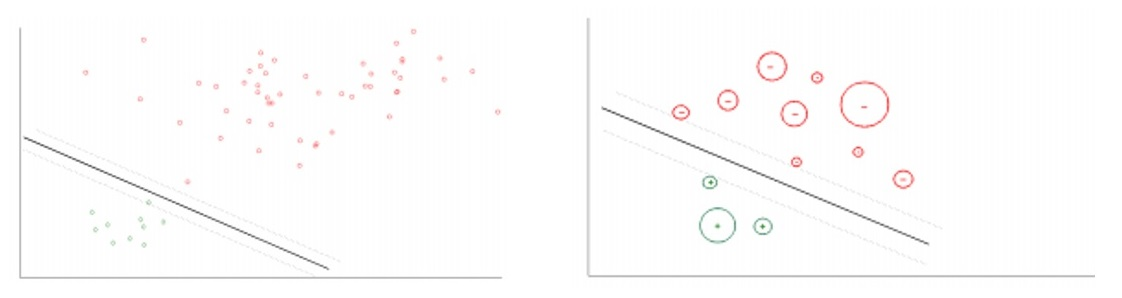
\includegraphics[scale=0.5]{snaps/socp.jpg}	
	\caption{Geometric interpretation for SVM and CBSOCP.\cite{socp}}
	\label{fig:socp}
\end{figure}
\begin{flushleft}
\textbf{Centrality-Aware Link Recommendations \cite{centrality} :}
\end{flushleft}

\indent This paper aims to reduce the closeness centrality of all nodes. They try to bring small world effect in the network where any node in the network can be reached from any node within few hops. They use existing link recommendations algorithms to suggest possible link formation to users where they aim on selecting those links such that closeness centrality of those nodes is reduced.
\begin{flushleft}
\textbf{Collective Prediction of Multiple Types of Links in Heterogeneous Information Networks \cite{collectiveprediction} :}
\end{flushleft}

\indent As conventional promixity measures fail to work on heterogeneous information network, they design a relatedness measure (RM) based on linkage homophily principle where two nodes can form a link if most of their similar nodes are linked together. They extend co-training method which handles label correlation between homogeneous network to heterogeneous network such that most confident predictions of unlabelled links are shared between the network.
\begin{flushleft}
\textbf{Handling Class Imbalance in Link Prediction Using Learning to Rank Techniques \cite{handlingclassimbalance} :}
\end{flushleft}

Due to the presence of large number of absent links, the misclassification error is not suitable for performance measure. Instead of misclassification error, many suggests to use ranking performance measures such as area under curve (AUC), average precision and normalized discounted cumulative gain (NDCG). This paper talks about link prediction as learning to
rank problem and they develop a link prediction method based on cross entropy surrogate used in ListNet ranking algorithm (Cao et al. 2007) \cite{listnet}.

\section{\textbf{Thermography}}

\indent Collective Classification is the problem of label predictions in the network. This problem finds many application in our day-to-day life like who influence other objects in the network, epidemiological network, predicting political affiliations and so on. Many real world data do not provide adequate label information, so this problem tends to be semi-supervised classification problem. This problems get more difficult when only a few labeled data is available. The semi-supervised learning method should be capable to handle this deficiency of labeled data. Label correlation is the key aspect in collective classification where the label of object $o$ can have correlation with that object's attribute or they can have correlation with the neighborhood attributes or they can have correlation with the unobserved labels in the neighborhood.
\begin{flushleft}
\textbf{Approximate Inference Algorithms for Approaches based on Local Conditional Classifiers :}
\end{flushleft}

%\indent There are two most commonly used approximate inference algorithms based on local conditional classifiers are :

Iterative Classification Algorithm (ICA) : This is an iterative algorithm where in each iteration, all unobserved nodes are taken and for those nodes in that iteration, we calculate the likelihood of the labels of a node based on its neighborhood labels predicted by the local classifier. We only assign a label to a node which has the maximum likelihood for that label. This iteration process can be continued till all class labels have been classified or till a threshold is reached.

Gibbs Sampling (GS) : The original algorithm of Gibbs Sampling is computationally expensive as they need to determine the convergence of the procedure. Thus an approximate version of gibbs sampling is proposed where they assume the conditional probability distribution given by the local classifier is correct. Gibbs sampling is very similar to ICA except that the number of iterations is initially fixed a to period called "burn-in". Once the burn-in period is reached, the algorithm start having a statistical count for each unobserved label, a count of labels assigned to the nodes. After certain sampling of the nodes, each node is assigned a label which has the maximum count from the statistical count.
\begin{flushleft}
\textbf{Multi-label Collective Classification in Multi-attribute Multi-relational Network Data\cite{priyesh} :}
\end{flushleft}

This paper is the one of the very few paper which handles multi-label classification in multi-attribute and multi-relational (MAMR) data. They propose a co-training style framework  which learns a classifier $(f^l)$ for each label (l $\epsilon$ L). The classifier $f^l$ can be break down into two classifiers $f^l_a$ and $f^l_g$ where the classifier $f^l_a$ is learned on each attribute view (a $\epsilon$ A) and the classifier $f^l_g$ is learned on each relational view (g $\epsilon$ G) separately. This is the minimization problem of the three loss functions $L_1 , L_2$ and $L_3$ where $L_1$ loss function is the loss on labeled data on both relational and attribute views. $L_2$ and $L_3$ loss functions updated in two steps in the co-training style proposed framework.
\begin{align*}
& min(\underbrace{L_1(A,G,L,T)}_{\text{Loss on labeled data}} + \underbrace{L_2(A,G,L,U) + L_3(A,G,L,U)}_{\text{Loss on unlabeled data}})\\
L_1(A,G,L,T) = & \sum_{l \in L}(\underbrace{\sum_{a \in A}\mathcal{L}(f_a^l(A_{T_l}^a),Y_{T_l}^l)}_{\text{Attribute views' disagreement}} + \underbrace{\sum_{g \in G}\mathcal{L}(f_g^l(G_{T_l}^g),Y_{T_l}^l)}_{\text{Relational views's disagreement}})\\
L_2(A,G,L,U) = & \sum_{l \in L}(\underbrace{\sum_{a \in A}(f_a^l(A_{U_l}^a) - \prod_{a \in A}f_a^l(A_{U_l}^a))^2}_{\text{Disagreemnet among attribute views}} + \underbrace{\sum_{g \in G}(f_g^l(G_{U_l}^g) - \prod_{g \in G}f_g^l(G_{U_l}^g))^2}_{\text{Disagreemnet among relational views}})\\
L_3(A,G,L,U) = & \sum_{l \in L}(\underbrace{\sum_{a \in A}(f_a^l(A_{U_l}^a) - \prod_{g \in G}f_g^l(G_{U_l}^g))^2}_{\text{Attribute views' disagreemnet with relational views}} + \underbrace{\sum_{g \in G}(f_g^l(G_{U_l}^g) - \prod_{a \in A}f_a^l(A_{U_l}^a))^2}_{\text{Relational views' disagreemnet with attribute views}})\\
\end{align*}
\subsection{\textbf{Network Embedding with Deep Learning Techniques}}
\begin{flushleft}
\textbf{Efficient estimation of word representations in vector space \cite{word2vec} : }
\end{flushleft}

This paper generally called as word2vec proposes two new log-linear models for learning distributed representations of words. In order to effectively minimize computational complexity caused by the non-linear hidden layer in the existing neural network language models (NNLM), they propose two simpler models which can be trained on large data more efficiently.

Continuous Bag-of-Words Model (CBOW) : This is similar to feedforward NNLM where non-linear hidden layer is removed and the projection layer is shared across all words. A log-linear model is built using few words from history and few words from future as input and the output is the current word. In general, the model will find the likelihood of the current word given those words.

Continuous Skip-gram Model (Skipgram) : This model is exactly opposite to CBOW model described above. Given the current word as input, it tries to maximize the likelihood of those words left and right to the current word. 

Hierarchical Softmax is used in the output layer as present in the typical NNLM but instead of balanced binary tree, huffman tree based hierarchical softmax is employed to give better computationally better speed up. As the embedding of the words are generated using anyone of the above two methods, one can do some simple algebraic operations between vectors and the resultant vector thus produced would be closer to the target word embedding. A simple architecture of these two models is shown in Fig \ref{fig:word2vec}. Example : Vector("King") - Vector("Man") + Vector("Women") is close to the word representation of the Vector("Queen").
\begin{figure}[!ht]
	\centering	
	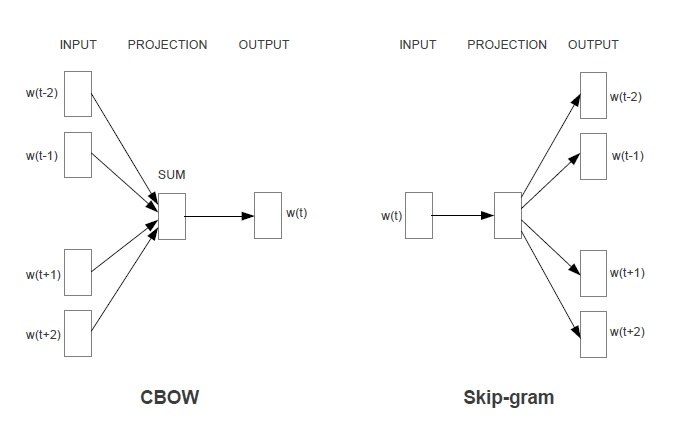
\includegraphics[scale=0.7]{snaps/word2vec.jpg}	
	\caption{The CBOW architecture predicts the current word based on the
context, and the skipgram model predicts the surrounding words given the current word \cite{word2vec}.}
\label{fig:word2vec}
\end{figure}
\begin{flushleft}
\textbf{Distributed Representations of Words and Phrases and their Compositionality \cite{word2vec2} :}
\end{flushleft}

This paper proposes several variants to skipgram model presented in Mikolov et al. \cite{word2vec}. They replace the complex hierarchical softmax used in the output layer with a simplified variant of noise contrastive estimation (NCE) called Negative Sampling (NEG). The Skipgram and the CBOW models do not need a full probabilistic model as achieved by hierarchical softmax, so they are trained using logistic regression where they try to discriminate the noise targets from real targets. Thus NEG samples \textit{k} words from the noise distribution and maximize the log likelihood of the target words. In addition to NEG, they proposed subsampling of frequent words. The main idea is that the frequent words like "the", "and" and "a" occurs millions of times and when they are added to words like "France" or "Paris", it doesn't makes the phrase meaningful. To avoid those words, each word is discarded with the probability,
\begin{align*}
P(w_i) = 1 - \sqrt{\frac{t}{f(w_i)}}
\end{align*}
where t is the threshold and f(w) is the frequency of the word.
\begin{flushleft}
\textbf{Heterogeneous Network Embedding via Deep Architectures \cite{hne} :}
\end{flushleft}

This paper mainly talks about data embedding where it is used to create low-dimensional feature representations by providing deep embedding algorithm for networked data. There are very few papers which talked about linking structural and content information using deep learning techniques. This paper does the same in completely supervised scheme. A non-linear multi-layered embedding function can capture linkage information and rich content and produce multi dimensional representation for an object in low dimensional space. After that, one generally need to feed it to any link prediction algorithm to solve it. This paper proposes heterogeneous network embedding (HNE) which maps the multi-attribute data to a unified latent representation. They learn embedding in three ways : i) They learn embedding between two images (node - node), ii) They learn embedding between texts of the same image (attribute - attribute) and iii) They learn embedding between image and texts of the same image (node - attribute). They use convolutional neural network to learn all these embedding where weights are shared between all these learning. Different embeddings are generated at these three learnings and then the way to combine the embeddings to form a single latent representation is unclear in the paper. They also proposed an extension of this architecture for MAMR data by stacking the relational matrices which they claim that it is not scalable for large graphs.

\begin{flushleft}
\textbf{DeepWalk: Online Learning of Social Representations\cite{deepwalk} :}
\end{flushleft}

Deepwalk learns latent representation of nodes in a graph by embedding the structural property of the nodes. On obtaining those embedding, one can perform off-the-shelf machine learning algorithms to perform link prediction, collective classification, anomaly detection, cluster analysis, etc. It gets the local information of the nodes by a series of short random walks performed at each node and then it is fed to the skipgram model proposed by Mikolov et al. \cite{word2vec, word2vec2}. The reason of choosing the  skipgram model is that the distribution of words appearing in natural language is similar to the distribution of vertices appearing in random walk which follows a power-law distribution.\\ This vertex representation modeling yields the following optimization problem :
\begin{align*}
min (\phi)~~~~~~- log Pr({v_{i-w},...,v_{i-1},v_{i+1},...,v_{i+w})}|\phi(v_i))
\end{align*}
where given a random walk sequence of a vertex, we need to find the probability of the other vertices occurring in that random walk. This increases the probability of the vertices in the neighborhood of the current vertex thus capturing the structural information of the graph. Once this model is trained with hierarchical softmax at output layer, the embedding are retrieved from the weight matrix in the projection layer.

\begin{flushleft}
\textbf{Author2Vec: Learning Author Representations by Combining Content and Link Information \cite{author2vec} :}
\end{flushleft}

This is a short paper where they extend deepwalk \cite{deepwalk} approach to learn both content and link information thus addressing single attribute single relational network data. They focus on co-authorship network where they learn embeddings for authors. They first learn content information of an author and then enrich that author's representation by capturing link information to get the final embeddings.

Content-Info Model : The textual content here is the abstract of the author and its feature representation is retrieved by paragraph2vec \cite{paragraph2vec} which converts paragraph to vector representation. This model gets the author's vector representation closer to the vector representation of the author's published papers whereas it deviates from other irrelevant papers' vector representation away from the author's vector representation.

Link-Info Model : This model is similar to the content-info model and it aims to bring the similarity between authors who published papers together closer in vector representation and the other authors away from it.
\begin{flushleft}
\textbf{Tri-Party Deep Network Representation\cite{triparty} :}
\end{flushleft}

This paper published in IJCAI-2016 is very similar to that of author2vec (WWW-16) \cite{author2vec} described above has an additional model designed to learn the labels of the vertices. In architecture wise, author2vec learns vertex representation in content-info model and then fed to link-info model, where as in this paper two embeddings are jointly learned in a coupled neural network model. The architecture of this model is given in Fig. \ref{fig:triparty}.\\
\begin{figure}[!ht]
	\centering	
	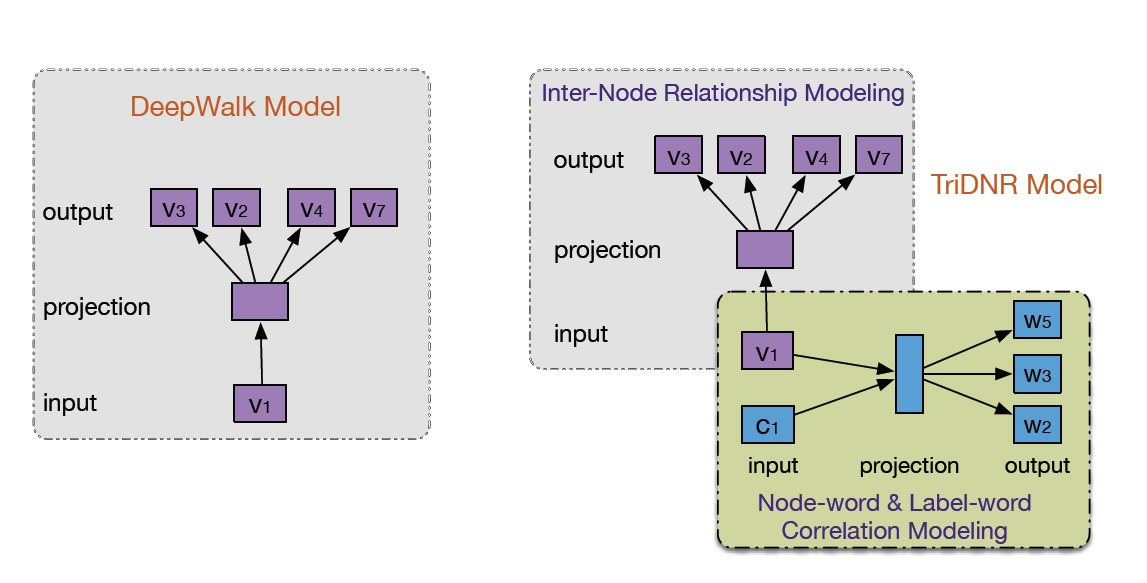
\includegraphics[scale=0.35]{snaps/triparty.jpg}	
	\caption{Architecture of Deepwalk model and TriParty model.\cite{triparty}}
	\label{fig:triparty}
\end{figure}
Inter-node Relational Modeling : It learns the embedding of the nodes given the series of random walk sequences of all nodes.

Node-content Correlations Assessing and Label-content Correspondence Modeling : Given a node and labels of its documents, it learns both the representation of its contents as well as the input label vectors. 

Connections : The two layers mentioned above are coupled together and the representation of nodes are learned together.

\begin{flushleft}
\textbf{Scaling up Link Prediction with Ensembles \cite{scale} :}
\end{flushleft}

This paper applies Non-Negative Matrix Factorization (NMF) in the ensemble decomposed components of the original graph such that it approximates the search space of possible link predictions to $O(n^2)$ comparisons. NMF for collaborative filtering algorithms are widely used in recommender systems for its effective prediction of score of any user with any item given the matrix is sparse. The authors have chosen Symmetric NMF of form, 
\begin{align*}
W = FF^T
\end{align*}
where the forbenious norm of $(W - FF^T)$ is minimized.

But the challenge in link prediction is that the adjacency matrix is very large when the number of nodes goes over million. To counter this problem, ensemble decomposition of the original graph is proposed such that applying Symmetric NMF over those decomposed components is feasible. Ensemble decomposition is now achieved by following sampling methods :

1. Random Node Bagging : Randomly select all nodes with probability $f$, where $f$ is the fraction of the graph to be broken and select all its neighbors.

2. Edge Based Bagging : It is similar to snowball sampling where they randomly select a node and its subsequent neighbors with probability 0.5 and this process repeats until the total number of nodes reaches the fraction $f$.

\section{\textbf{Machine Learning}}

\subsection{\textbf{Support Vector Machines}}
\subsection{\textbf{Convolutional Neural Networks}}
\subsection{\textbf{Autoencoders}}
\subsection{\textbf{Segmentation /  Object Detection / Object localization}}

\subsubsection{\textbf{Optical Flows}}